\section{Introduction}
The discovery of a Higgs-like boson at the
LHC~\cite{ATLAS_higgs,CMS_higgs} was the first step toward a better
understanding of the electroweak symmetry breaking (EWSB)
mechanism. One important, and unverified, prediction of the Standard
Model (SM) is that the scattering amplitude of longitudinal vector
bosons ($V_{L}V_{L} \rightarrow V_{L}V_{L}$) is unitarized by the
Higgs boson.  Measuring VBS processes at a hadron collider, however,
is experimentally challenging. The ATLAS and CMS collaborations
recently provided the first evidence for and study of a VBS process
using events with two same-electric-charge $W$ bosons in association
with two forward jets ($pp \to$ \ssWW)~\cite{ATLAS_ssWW,CMS_ssWW}.
This final state has the advantage of relatively small SM background
contributions compared to other VBS processes, paired with a
production rate large enough to measure in early LHC datasets.  While
an ideal candidate for first observation of the VBS process, measuring
the longitudinal fraction of these events is not straight forward.

In general the polarization of a gauge boson can be determined from
the angular distribution of its decay products.  Since a $W$ boson
only couples to left-handed particles and right-handed
anti-particles. In the rest frame of the $W$ boson, the decayed
charged lepton is expected to preferentially pointing in the $W$ boson
spin direction for $W^+$ and in the opposite $W$ boson spin direction
for $W^-$. {\bf Two sentences are disconnected - what are you trying to say?
Preferred emission depends on W helicity states...} The normalized differential cross section of a
leptonically-decaying $W$ boson can be written in terms of
polarization fractions as~\cite{}:
\begin{multline}
 \frac{1}{\sigma} \frac{d\sigma}{d\cts} = \frac{3}{8} f_- (1 \mp \cts)^2 + \frac{3}{8} f_+ (1 \pm \cts)^2 \\ 
+\frac{3}{4} f_L (1 - \ctsSq) , {\text {for~}} W^\pm 
\end{multline}
%  R. Ellis, W. Stirling, and B. Webber, QCD and collider physics
%, Camb. Monogr. Part. Phys. Nucl. Phys. Cosmol. 8 (1996) 1
where \ts is the angle between the charged lepton in the $W$ boson
rest frame and the $W$ boson direction of motion.  The three fraction
parameters $f_{-}$, $f_{+}$ and $f_L$ denote the fractions of $W$
events with three possible helicity states $-1$, $+1$ and 0,
respectively.  They are constrained via $f_- + f_+ + f_L = 1$.  In
order to measure \ts, we need to fully reconstruct the direction of
motion of the $W$ boson.

Requiring both $W$ bosons to decay leptonically in the $pp
\to$ \ssWW events enables the determination of the charge of
each $W$ boson via the charged leptons. However, since the
corresponding two neutrinos in the final state escape detection, the
$W$ boson rest frames cannot be directly measured.  It is thus
difficult to determine the polarization fractions of each boson and
the fraction of longitudinal scattering events in the \ssWW process.

Many proposals have been made to determine the longitudinal scattering
fractions in other VBS final states, such as semi-leptonic
$WW$~\cite{Han:2009em} {\bf How does the hadronic W charge assignment
  work?}, $WZ$~\cite{aa} and $ZZ$~\cite{le houche report} or
fully-leptonic decay modes of $WZ$ and $ZZ$ scattering, where the full
event kinematics can be reconstructed. However, these channels either
suffer from large SM backgrounds not present in the \ssWW channel or
have relatively low production cross sections. Attempts have been made
to gain sensitivity through other variables than \ts in the \ssWW
channel. One example is the variable $R_{p_T}=(p_{T}^{\ell 1} \times
p_{T}^{\ell 2}) / (p_T^{j_1} \times p_T^{j_2})$~\cite{Doroba:2012pd},
where $\ell_1$ and $\ell_2$ denote the two leptons in no particular
order and $j_1$ and $j_2$ denote the two most energetic jets in the
event.  It is natural to assume that not all of the sensitivity to
longitudinal scattering is encompassed in a single variable, and that
better discrimination could be obtained by combining the available
event information with a machine learning technique. In this paper we
develop a method to use a neural network to map measurable quantities
to the truth \cts values that contain the polarization information of
the two $W$ bosons.

\section{Machine learning model}
While it has become common practice in high energy physics to use
multi-variate techniques to separate signal from background, to the
author's knowledge multi-variate regression has not been used to
directly predict underlying quantities {\bf also not in H
  properties?}.  Recent success with deep learning in other areas of
HEP~\cite{Baldi:2014pta,Baldi:2014pta} {\bf ???incomplete sentence}.

For the \ssWW events, we use representative measurable quantities such
as the transverse momentum ($p_T$), pseudorapidity ($\eta$) and
azimuthal angle ($\theta$) {\bf you mean polar angle theta or
  azimuthal angle phi? I assume the latter bc. we use theta in eta
  already.} of the two leptons and two jets, and $x$ and $y$
components of the missing transverse energy ($\slashed{E}_T^x$ and
$\slashed{E}_T^y$).  Thus, the overall number of measurable quantities
we use is 14. The goal of the multi-variate technique is then to find
the best mapping from these measurable quantities to the two truth
values of \cts (one for each $W$ boson) present in each event.  We
choose a multi-layer neural network with a final output layer with
linear activation. The neural network was implemented with the Theano
software packages~\cite{theano}. Hyper-parameters were tuned by hand,
but undoubtedly could be improved.  The cost function is defined as
the mean error squared: \small
\begin{equation}
{\cal{C}}= \sum_{i=1}^{N} [(\ctsnb_{1,i} -N_{1,i})^2+(\ctsnb_{2,i}-N_{2,i})^2]/2N
\end{equation}
\normalsize where $N$ is the overall number of events used,
$\ctsnb_{1/2,i}$ is the truth value of \cts for each $W$ boson with
random ordering for the $i$-th event, and $N_{1,2/i}$ is the value of
the two neural network outputs.  The stochastic gradient descent
algorithm~\cite{sgd} is used to find all weights and biases in the
neural network that minimizes the overall cost function using a
training sample.

We generate *** \ssWW events using the {\sc madgraph} event
generator~\cite{madgraph} at a proton-proton center-of-mass energy of
13 TeV.  The NN23l01 {\bf this is the MG internal name - use the full
  name?} parton distribution function~\cite{pdf} is used as the
default. {\bf PS used? Pythia?} To emulate the behavior of a typical
general-purpose LHC detector, these events are then passed through the
detector response simulation of the ATLAS detector implemented in {\sc
  delphes}~\cite{delphes}. {\bf mention jet alg/size etc. here} Events
are split into three categories: 1/4 are used in a training sample,
1/4 are used for a validation test against over-training, and the
remaining 1/2 are used to build templates and do sensitivity
studies. A ** layer neural network with ** hidden neurons and a
learning rate of ** is used.

%\begin{figure}
%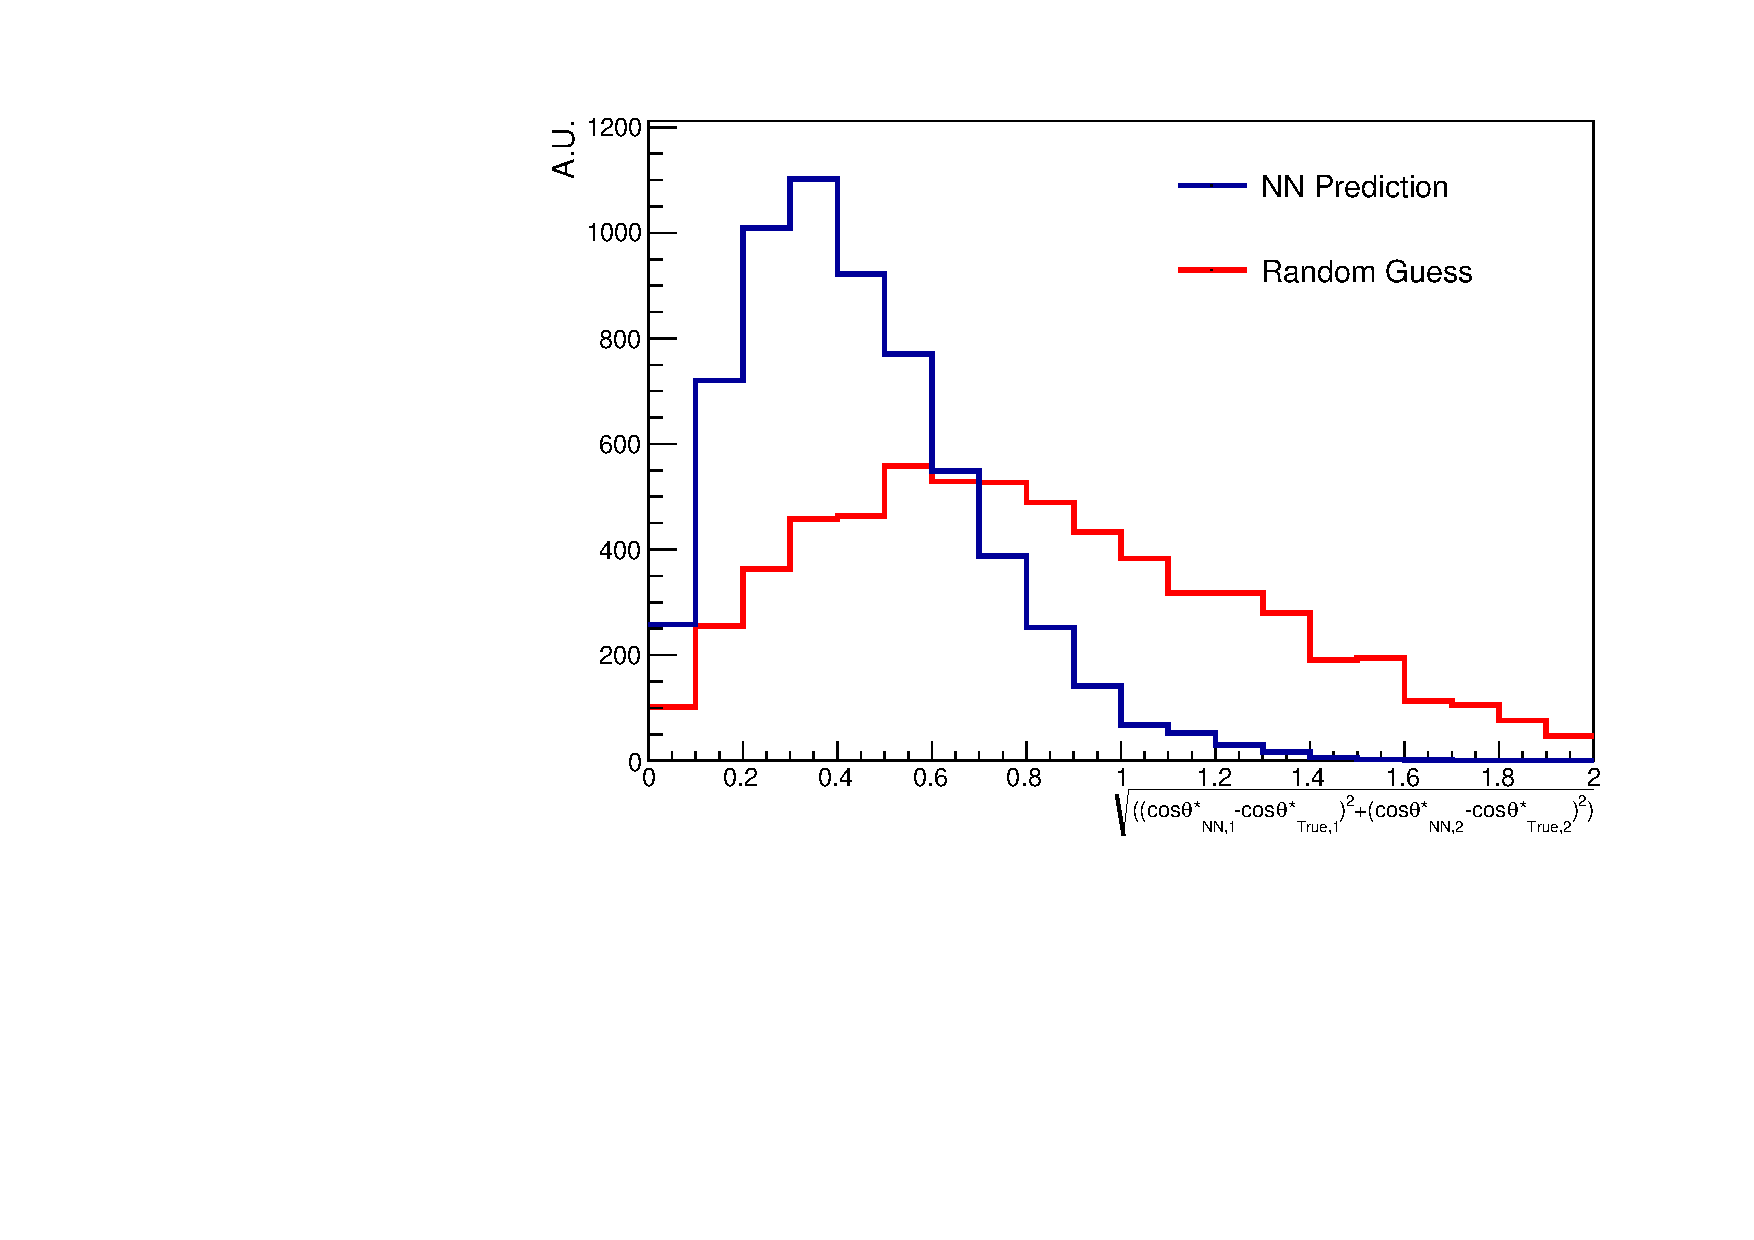
\includegraphics[width=.45\textwidth]{./fig/OneD_cts_compare.pdf}
%\caption{\label{fig:mlp_err} Distance of prediction from the true value of ($\ctsnb(1)$,$\ctsnb(2)$)}
%\end{figure}

\section{\label{sec:signal} Signal Model}
To reduce the contributions from other SM processes, we apply the
following generator level cuts on the \ssWW sample:
\begin{itemize}
\item Quark $p_T > 20$ GeV and $|\eta| < 5$;
\item Lepton $p_T > 10$ GeV and $|\eta| < 2.5$;
\item $\dR_{jj}>0.4$, $\dR_{\ell \ell}>0.4$ and $\dR_{\ell, j} > 0.4$;
\item Invariant mass of the two quarks $M_{jj}> 150$ GeV.
\end{itemize}
The resulting cross section at 13~TeV is 8.4~fb, which is used to
normalize the expected number of signal events.

We will first demonstrate the usefulness of deep learning networks
with this general sample and then discuss the effects of cuts to
reject other backgrounds as well as detector modeling effects.  {\bf
  so this is at truth level before delphes, and no cuts applied?  Need
  to better define ``general/default/original'' here and below.}

Polarization fractions are first obtained on the default sample by
fitting the two-dimensional distribution of the truth \cts variable
for each $W$ boson.  In order to fit for these polarization fractions
templates must be built for ``pure'' polarization states. These
templates are created by reweighting each event based on the truth
\cts distribution. The weight $W_i$ for the $i$-th event is given by
$W_i = F_i/n_i$, where $n_i$ is used for the normalization and is
defined as
\begin{multline}
n_i=[ \frac{3}{8} f_- (1 \mp \ctsnb_1)^2 + \frac{3}{8} f_+ (1 \pm \ctsnb_1)^ 2 +\frac{3}{4} f_L (1 - \ctsSqnb_1)] \\
\times [ \frac{3}{8} f_- (1 \mp \ctsnb_2)^2 + \frac{3}{8} f_+ (1 \pm \ctsnb_2)^ 2 +\frac{3}{4} f_L (1 - \ctsSqnb_2)]. 
\end{multline}
The $F_i$ represent the six possible polarization states for the two
$W$ bosons: Left-Left ($--$), Left-Right ($-+$), Right-Right($++$),
Left-Longitudinal ($-L$), Right-Longitudinal ($+L$), or
Longitudinal-Longitudinal ($LL$). They are defined as \small
\begin{equation}
F_i \in  \left( \begin{array}{c} 
  --=f_-^2 (1 \mp \ctsnb_1)^2(1 \mp \ctsnb_2)^2,\\
  -+=f_- f_+[ (1 \mp \ctsnb_1)^2(1 \pm \ctsnb_2)^2\\ \;\;+(1 \pm \ctsnb_1)^2 (1 \mp \ctsnb_2)^2],\\
  ++=f_+^2 (1 \pm \ctsnb_1)^2(1 \pm \ctsnb_2)^2,\\
  -L=f_- f_L[ (1 \mp \ctsnb_1)^2(1 - \ctsSqnb_2)\\  \;\;+(1 - \ctsSqnb_1))(1 \mp \ctsnb_2)^2 ],\\
  +L=f_+ f_L[ (1 \pm \ctsnb_1)^2 (1 - \ctsSqnb_2))\\  \;\;+(1 - \ctsSqnb_1)(1 \pm \ctsnb_2)^2 ],\\
  LL=f_L^2 (1 - \ctsSqnb_1))(1 - \ctsSqnb_2)\\
\end{array} \right).
\end{equation}
\normalsize Since no ordering is applied to the two bosons we require
that the individual polarization fractions $f_-$,$f_+$,$f_L$ are the
same for both $W$ bosons.  For reweighting the original sample $f_-$,
$f_+$, $f_L$ are take as a function of the invariant mass of the
diboson system ($M_{WW}$).  Weights are calculated before any
additional event level cuts are made, and the resulting templates are
remade for each set of cuts explored.  To validate the reweighting
procedure, we also generate pure polarization state samples using {\sc
  madspin} and compare the obtained events kinematics with those
obtained from the reweighted sample. {\bf Does this mean you got the
  MG5 scripts to work and add the helicity to the lhe?}
Figure~\ref{fig:2D_polarization_six} shows the calculated $\cts_1$ vs
$\cts_2$ distribution for all six polarization states.

\begin{figure}
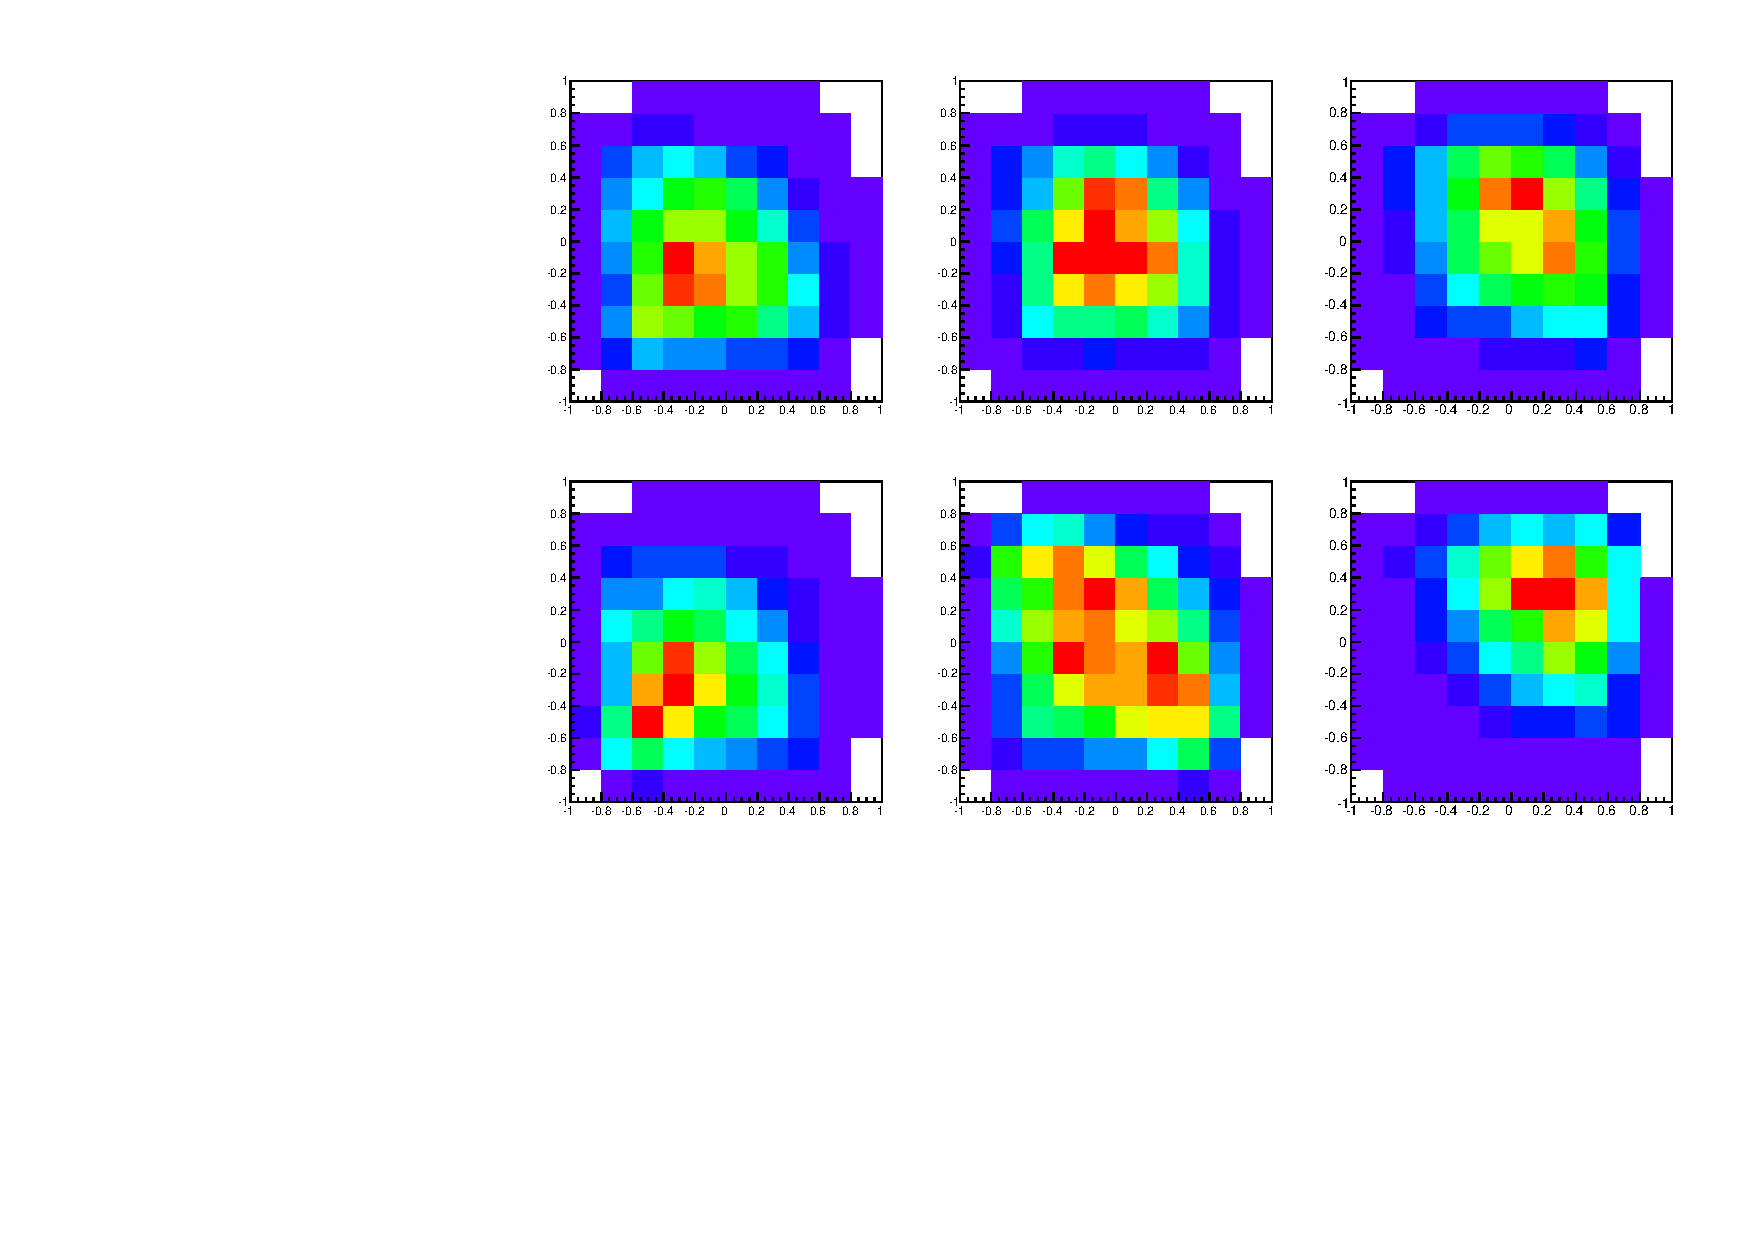
\includegraphics[width=.49\textwidth]{./fig/2D_temps.pdf}
\caption{\label{fig:2D_polarization_six}Two-dimensional $\cts_1$
  vs. $\cts_2$ templates after reweighting to pure polarization states
  which are clock-wise starting from the upper left:
  LO,OO,RO,LL,LR,RR. {\bf nomenclature: L is left here, longitudinal
    in eq. 4? Need axis labels, larger figure...}
\end{figure}
 

We combine events with both $W$ bosons transversely-polarized as
``$TT$'' (the sum of $--$, $-+$ and $++$ combinations), events with
one $W$ boson transversely-polarized and one $W$ boson
longitudinally-polarized as ``$TL$'' (the sum of $-L$ and $+L$
combinations), and events with both $W$ bosons
longitudinally-polarized as ``$LL$''. This allows to better constrain
the $LL$ scattering fraction of interest, under the assumption that
the relative admixture of contributions within $TT$ and $TL$ does not
change. Figure~\ref{fig:2D_polarization_three} shows the calculated
$\cts_1$ vs $\cts_2$ distribution for these three polarization states.
{\bf random remark: these dists seem symmetric wrt. the 45 deg
  bisector?  If so, one could gain stat power by adding both halves up
  and using halved templates?}

\begin{figure}
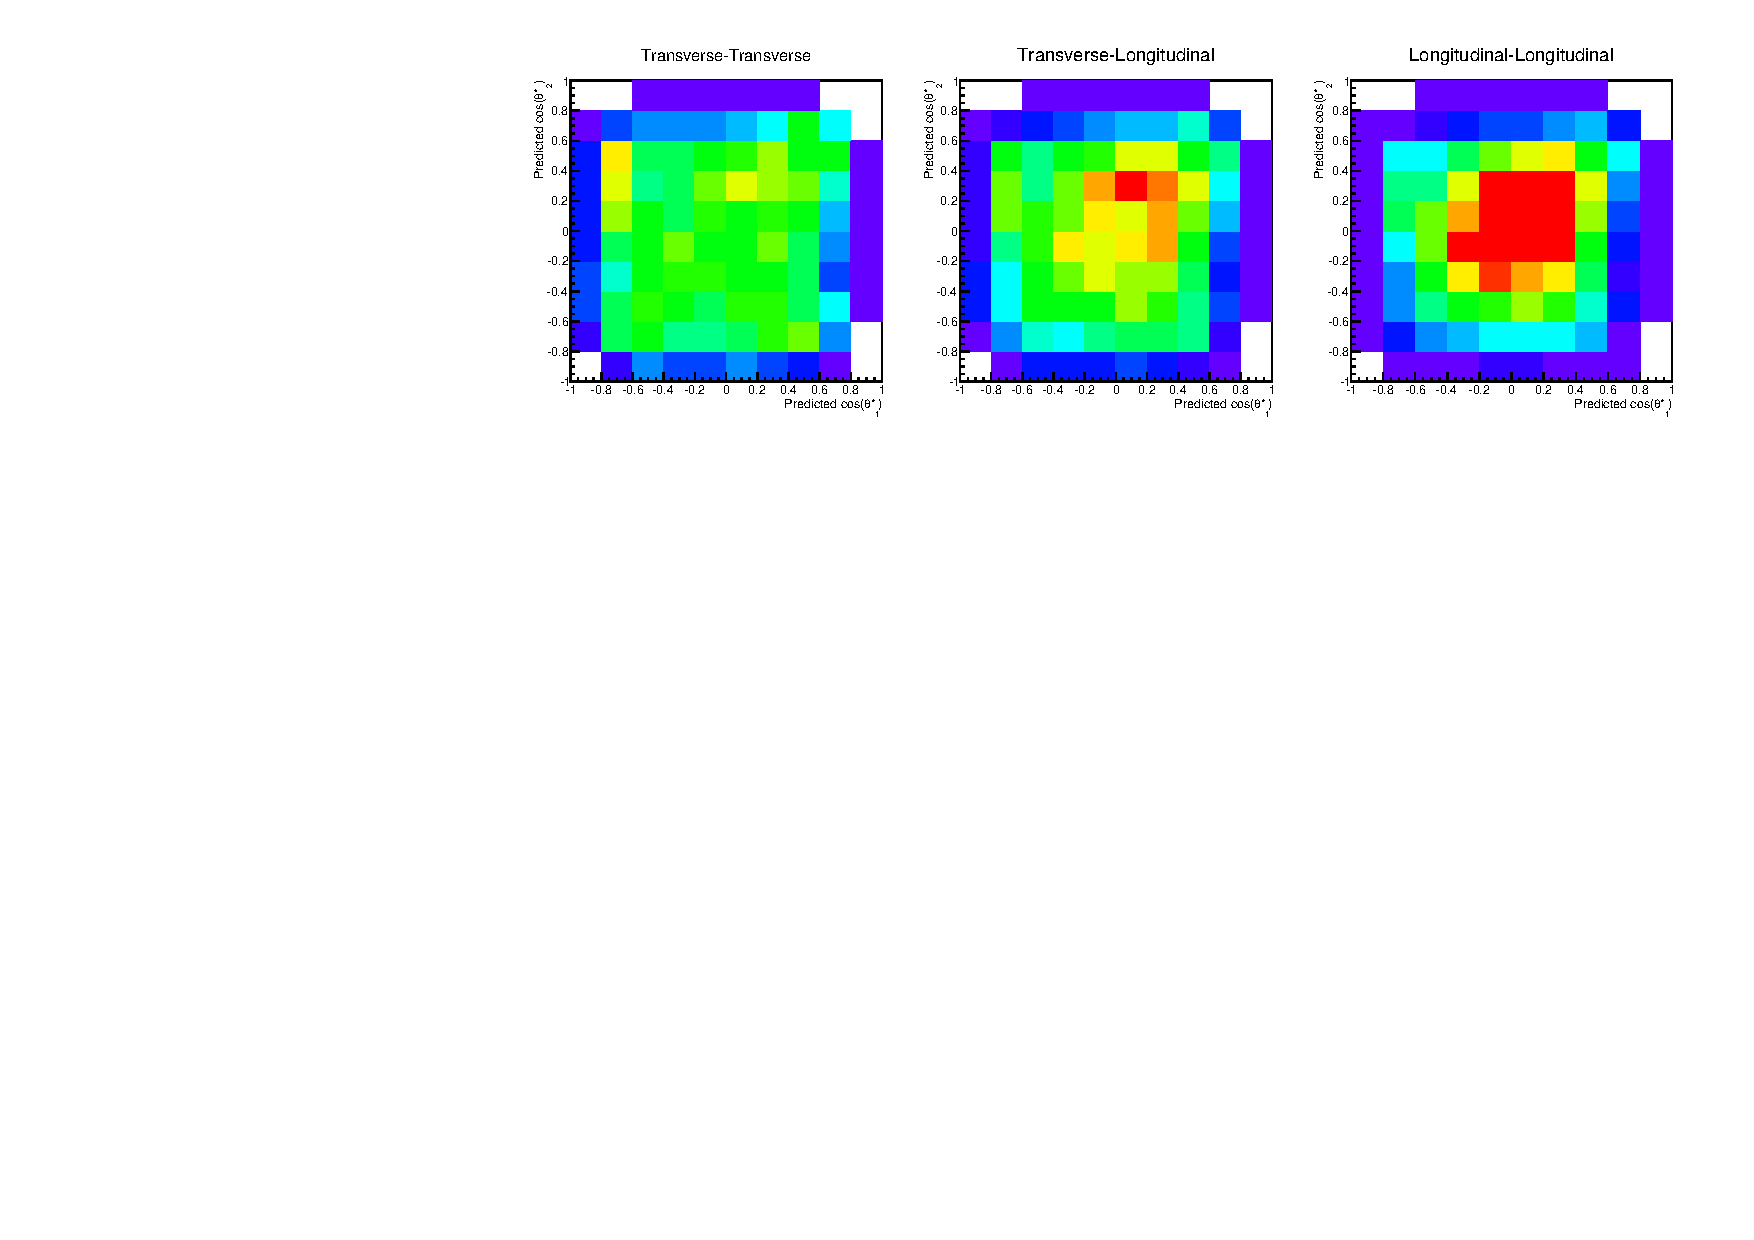
\includegraphics[width=.49\textwidth]{./fig/templates.pdf}
\caption{\label{fig:2D_polarization_three}Two-dimensional $\cts_1$ vs.
  $\cts_2$ templates after reweighting to the three polarization
  states $TT$ (left), $TL$ (middle) and $LL$ (right).}
\end{figure}

Figure~\ref{fig:Rpt} shows the normalized $R_{p_T}$ templates for
these three polarization states. The differences at large $R_{p_T}$
indicate the sensitivity of this variable to different polarization
states.
\begin{figure}
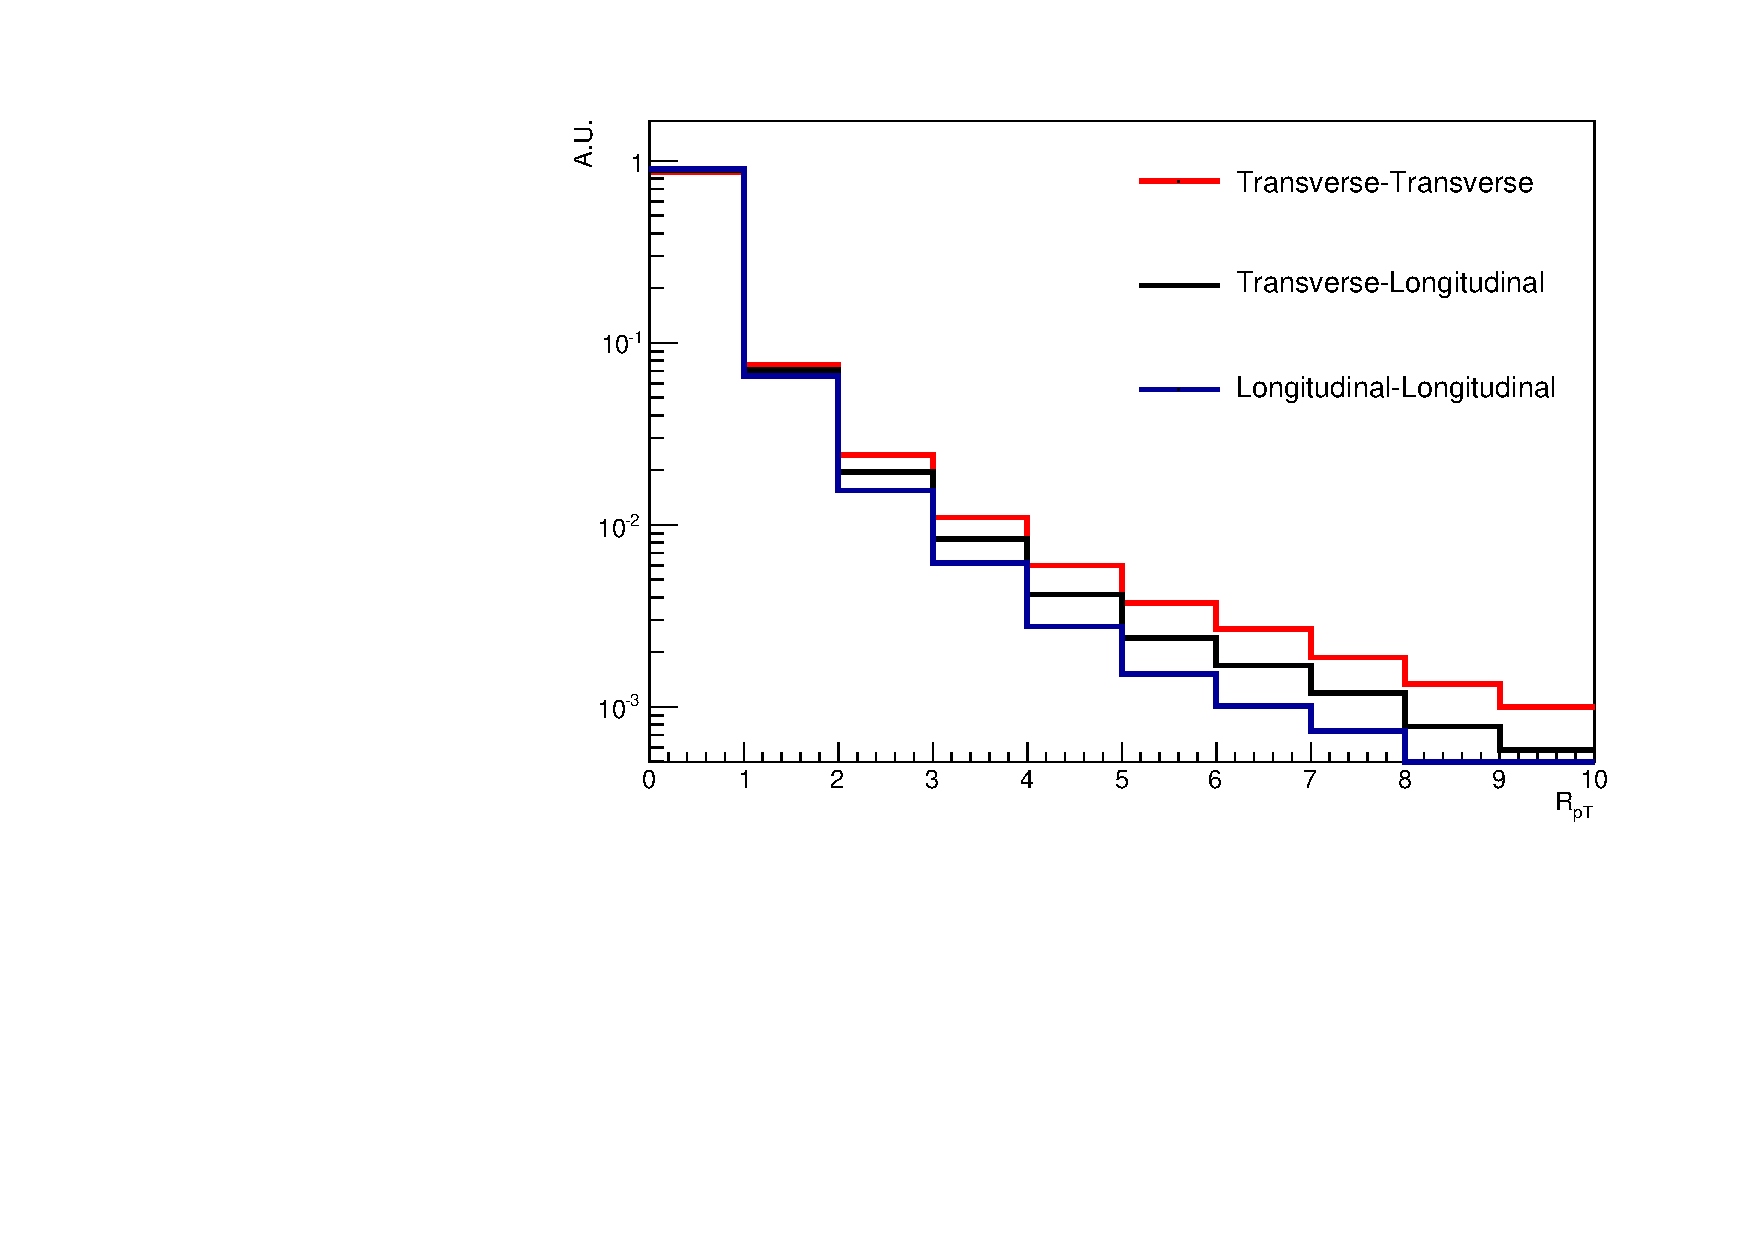
\includegraphics[width=.45\textwidth]{./fig/templates_2D.pdf}
\caption{\label{fig:Rpt}$R_{p_T}$ templates for three polarization
  states: $TT$, $TL$ and $LL$. {\bf is the legend correct? I thought
    LL is between TL, TT?}
\end{figure}

\section{Results}

Having established templates for each polarization state and a
distribution that is sensitive to different polarization states, all
we have to do is fit the resulting calculated $\cts_1$ vs $\cts_2$
two-dimensional distribution in data to derive each polarization
fraction.  In actual data analysis, this would involve first selecting
events to remove SM backgrounds and then subtracting predicted
background from data.  The effect of additional selection criteria and
backgrounds is covered below, but for the case of this section we
assume that {\sc madgraph} selection can be fitted directly to obtain
sensitivities.  A maximum likelihood fit is performed with the RooFit
framework~\cite{aa}. Fit uncertainties are determined by randomly
fluctuating data expectations within their Poisson errors and
repeating the fit, and confidence intervals are derived from the toy
experiments.  To validate the fitting method, we also make sure the
fitted values for each fraction agree with with the values obtained at
the truth level. {\bf transition from truth level templates to reco
  level dists not clear; where has NN been used?}

The precision for all six polarization fractions as a function of the
integrated luminosity are presented in Fig.~\ref{fig:sen_6}.  The
corresponding precision by fitting the $R_{p_T}$ distributions are
also shown for comparison. Better precision is obtained for the
calculated $\cts$ variables, which indicates that it is a more
sensitive variable to different polarization states than $R_{p_T}$.
The precision for the LL fraction is **\% (**\%) for an integrated
luminosity of 100 (3000) fb$^{-1}$, to be compared with **\% (**\%)
when using $R_{p_T}$.

The precision for the three combined polarization fractions $TT, LT,
LL$ as a function of the integrated luminosity are presented in
Fig.~\ref{fig:sen_3}.  The corresponding precision by fitting the
$R_{p_T}$ distributions are also shown for comparison. As expected,
better precision can be obtained by reducing the number of templates
used.  Transverse components can be measured with great precision,
whereas separating pure longitudinal-longitudinal scattering from
longitudinal-transverse scattering is challenging. However, if we fix
the TL fraction to the SM prediction, we can perform a precise
measurement of the LL fraction, as shown in Fig.~\ref{fig:sen_2}. In
all cases the neural network output outperforms the $R_{pT}$ variable
by **\% or more. {\bf fix TL to SM or use TT+LT+LL=1 ?}

\begin{figure}
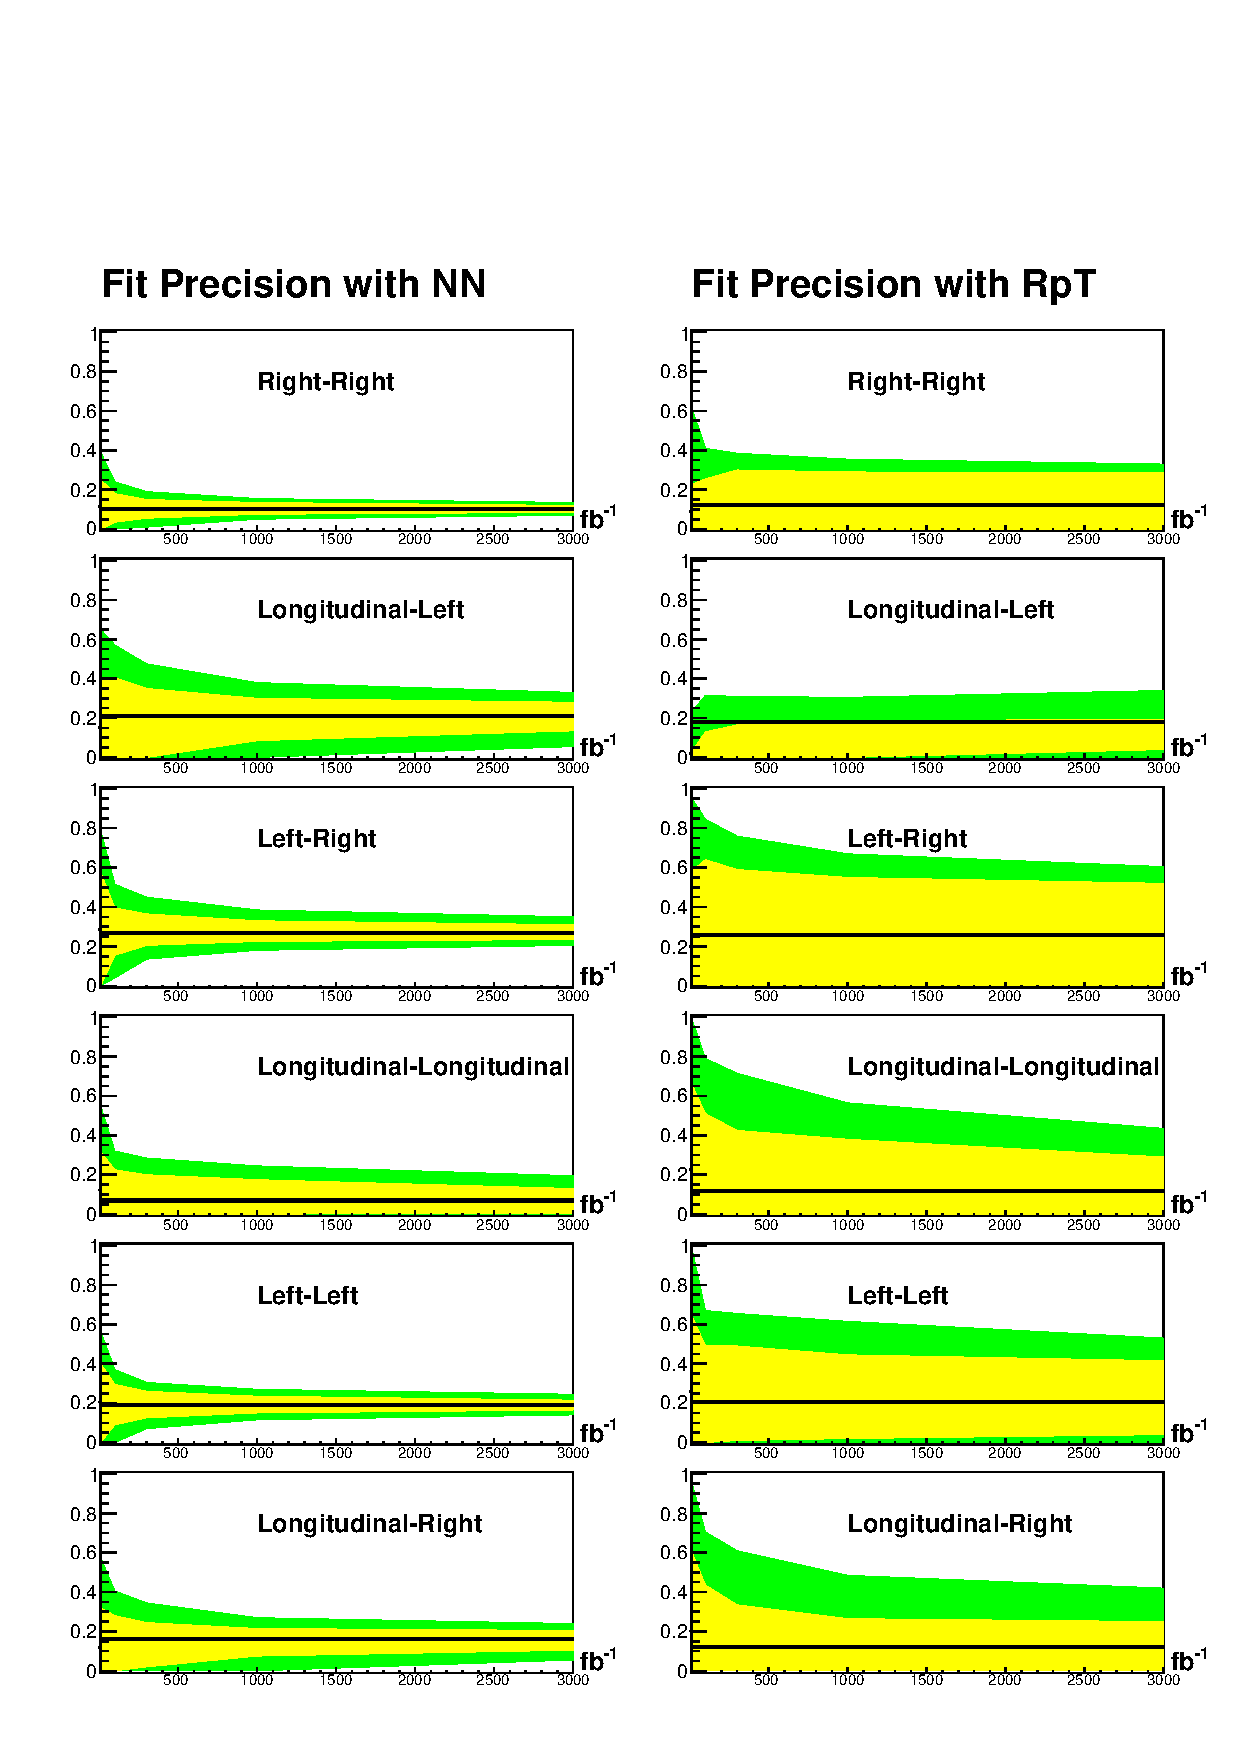
\includegraphics[width=.45\textwidth]{./fig/sens_0.pdf}
\caption{\label{fig:sen_6} 68\% and 95\% confidence intervals for fits
  with six polarization templates as a function of integrated
  luminosity. Fits are shown for the neural network on the left and
  for $R_{pT}$ on the right.}
\end{figure}

\begin{figure}
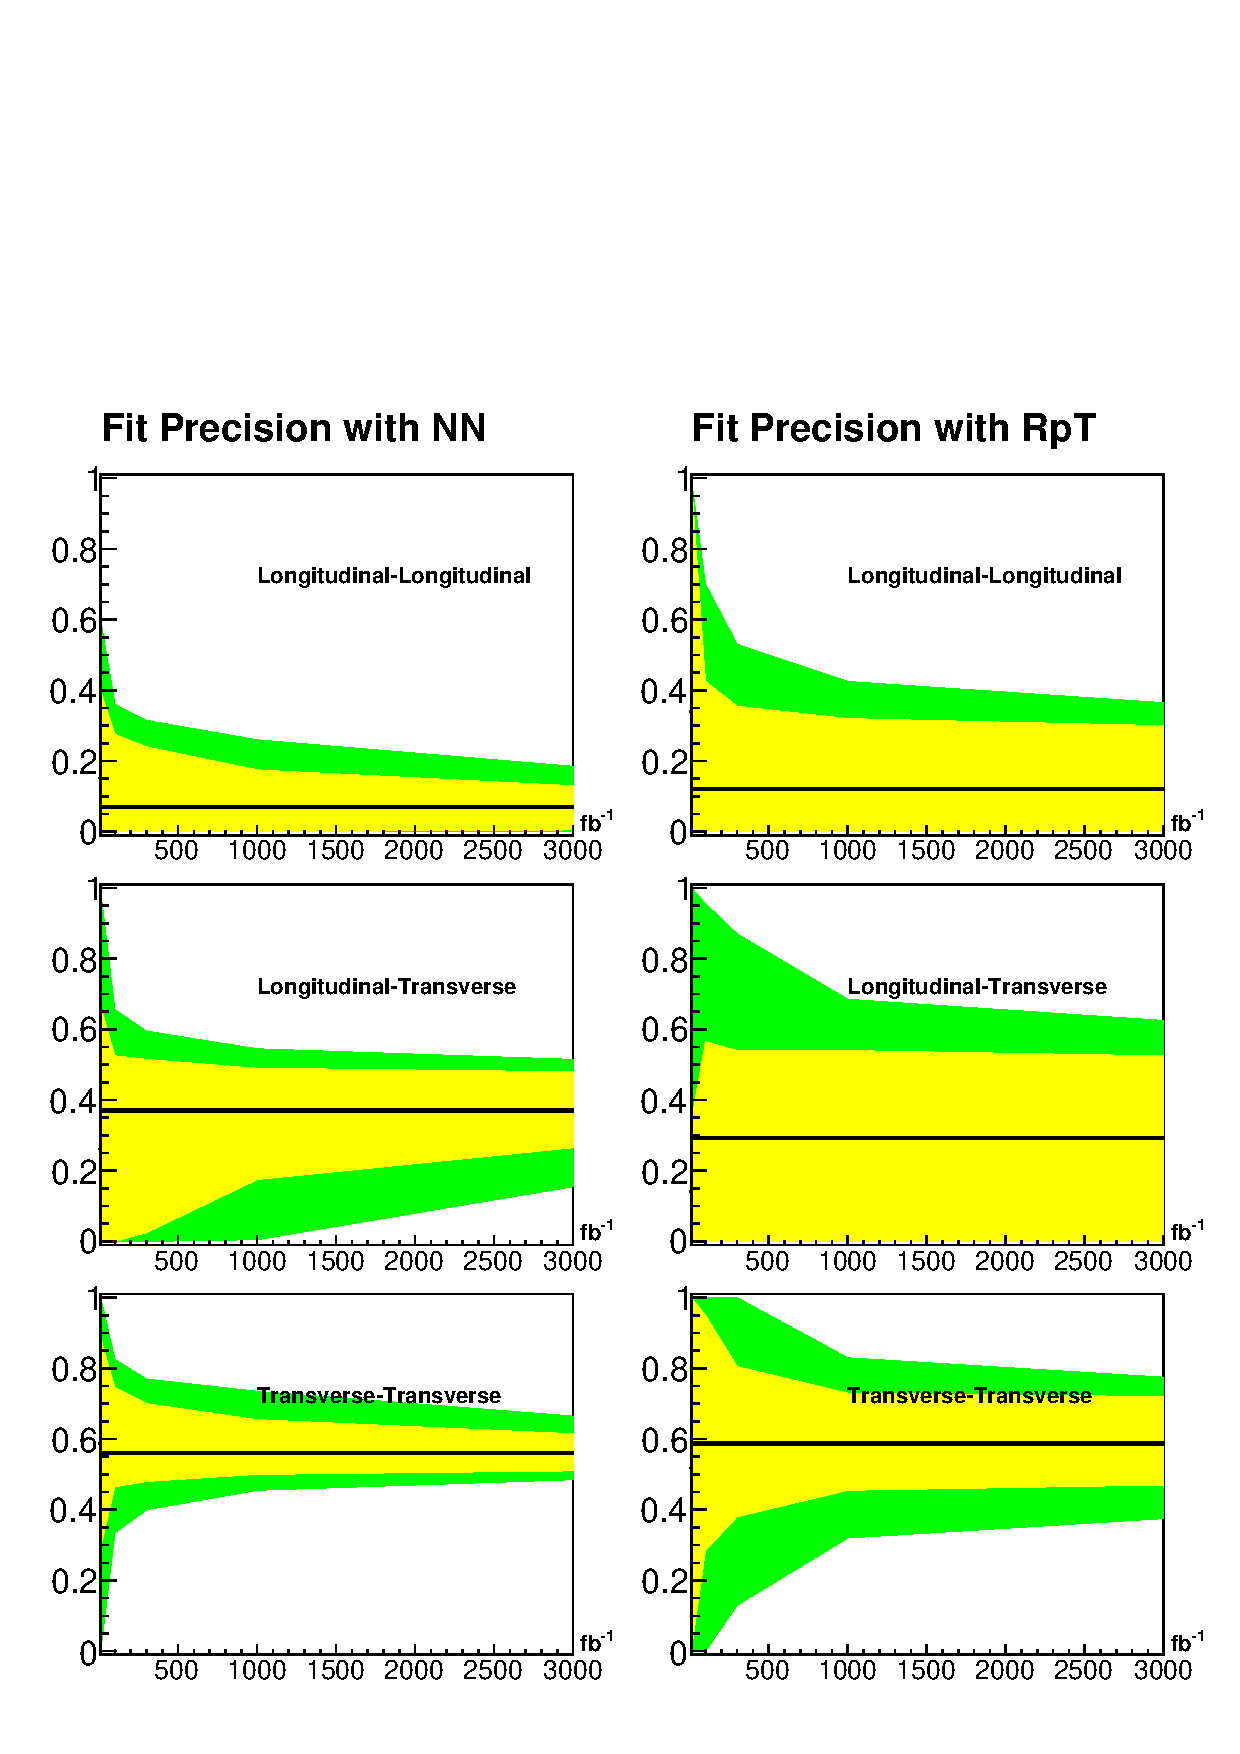
\includegraphics[width=.45\textwidth]{./fig/sens_1.pdf}
\caption{ \label{fig:sen_3} 68\% and 95\% confidence intervals for
  fits with three polarization templates as a function of integrated
  luminosity. Fits are shown for the neural network on the left and
  for $R_{pT}$ on the right.}
\end{figure}

\begin{figure}
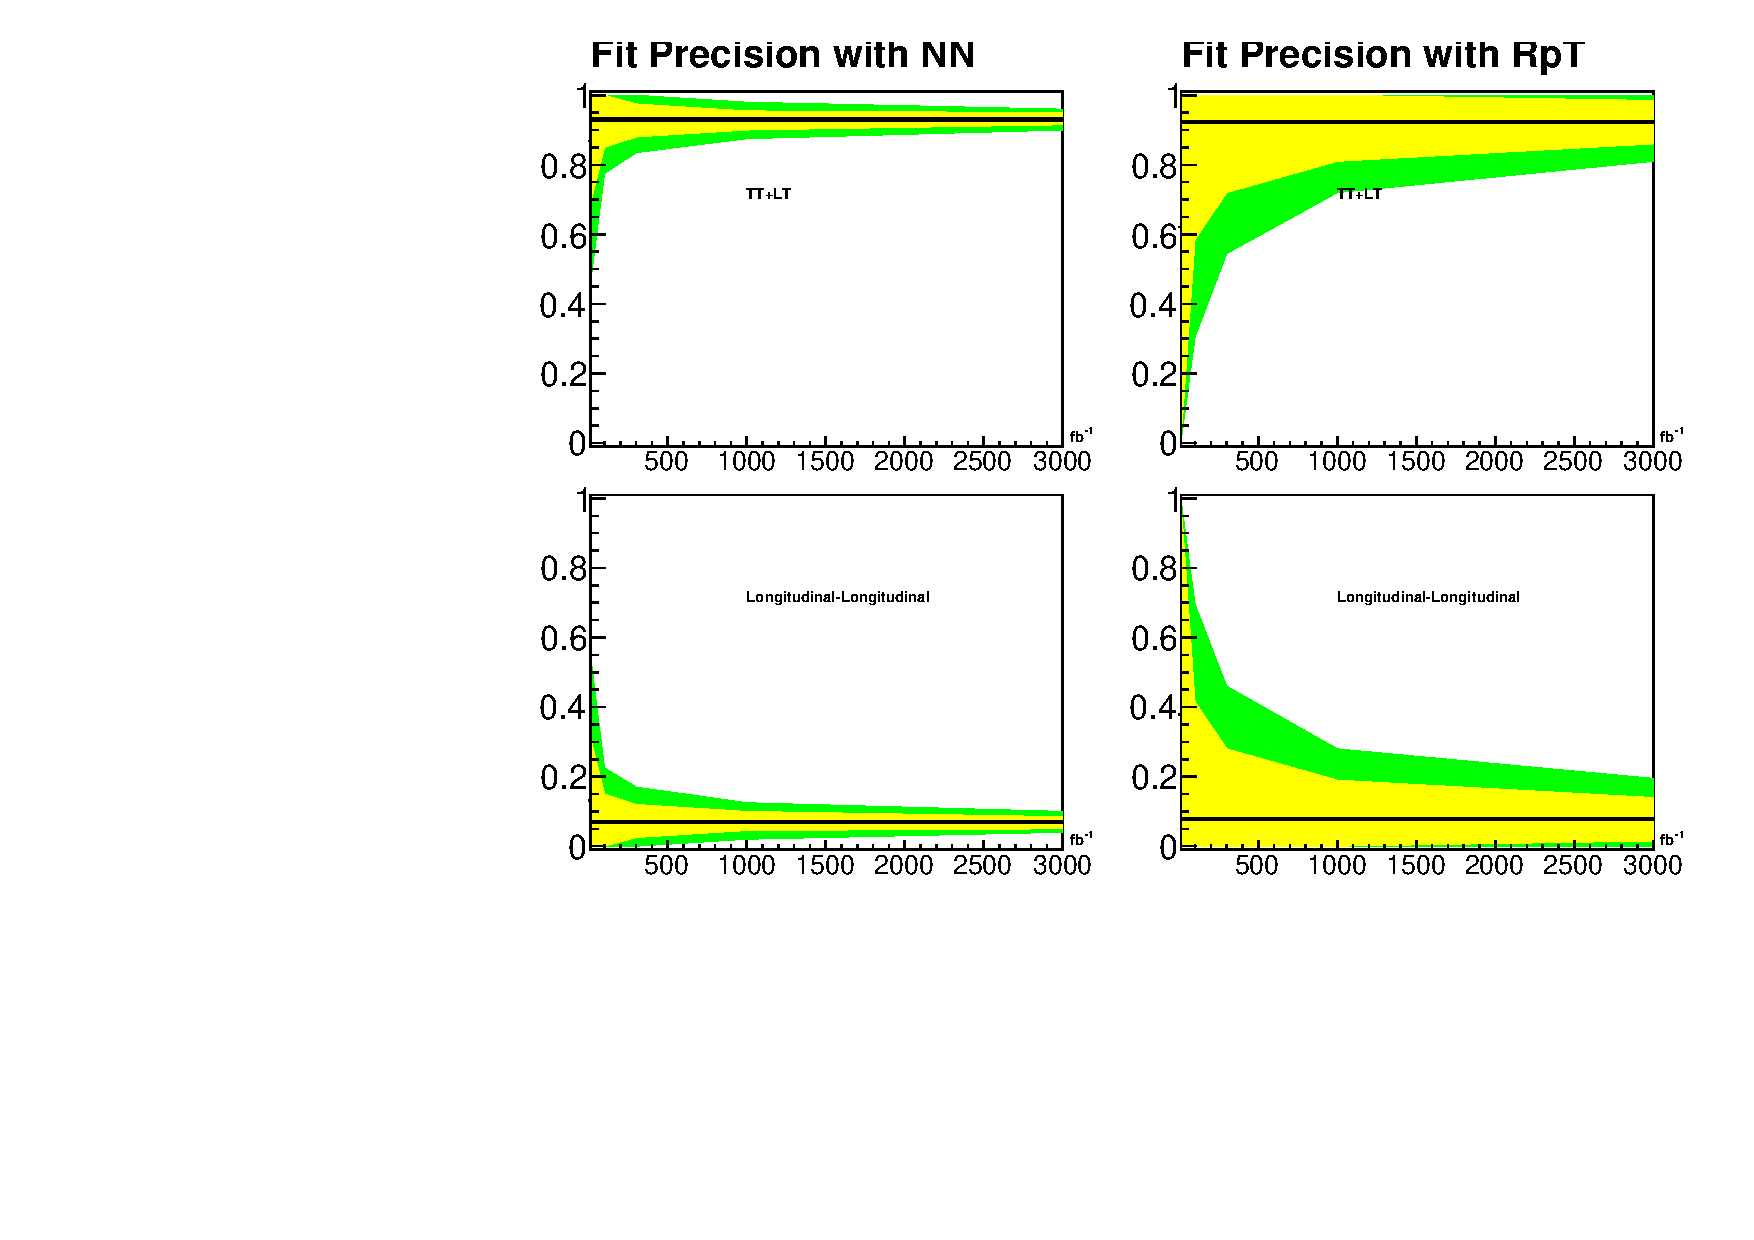
\includegraphics[width=.45\textwidth]{./fig/sens_2.pdf}
\caption{\label{fig:sen_2} 68\% and 95\% confidence intervals for fits
  with two polarization templates as a function of integrated
  luminosity. Fits are shown for the neural network on the left and
  for $R_{pT}$ on the right. {\bf if you use TT+LT+LL=1 you also end
    up with two independent pars only to fit...}}
\end{figure}

While the success of this neural network at the parton level is
encouraging, it is important to check if this procedure will stand up
to experimental realities of finite detector resolution and non-VBS
background. To reduce SM backgrounds in the loose fiducial region as
defined in Sect.~\ref{sec:signal} , we apply similar {\bf additional}
cuts as used by the ATLAS collaboration~\cite{ATLAS_ssWW} to obtain a
tight fiducial region:

\begin{itemize}
\item Jet $p_T > 30$ GeV;
\item Lepton $p_T > 25$ GeV;
\item $\slashed{E}_T > 40$ GeV;
\item $M_{jj} > $500 GeV;
\item $|\Delta Y_{jj}| > 2.4 $.
\end{itemize}

After the application of these cuts the dominant background comes from
$WZjj$ production where one lepton is not detected or not
reconstructed.  For the generated \ssWW events, we also use {\sc
  pythia6} for parton shower and hadronization simulation and then
pass these events through the {\sc delphes} package (using the CMS
simulation card)~\cite{delphes} to simulate the detector response of a
general-purpose particle detector at the LHC {\bf repeat from above,
  rm once. Maybe easier to follow if first parton level studies are
  shown and then delphes?}.  We define the loose and tight fiducial
regions at both the parton level and also at the {\sc delphes} level.
Table~\ref{tab:sens} shows the extracted limits on TT, TL and LL
fractions for loose and tight fiducial regions defined at the parton
level and at the {\sc delphes} level.  Table~\ref{tab:sens2} shows the
corresponding numbers on TT$+$TL and LL fractions.  An integrated
luminosity of ** fb$^{-1}$ is assumed.

Figure~\ref{sig_bkg} shows the calculated {\bf I removed
  ``calculated'' a couple times now, but you likely want to imply with
  it that it stems from the NN? Need to come up with proper labeling}
$\cts$ distribution for the dominant $WZ$ background, $++$ and $LL$
{\bf figure caption/legend contradict text: ++ vs. RR, AllSM vs. ??}
components of the \ssWW events.  It can be seen that the calculated
$\cts$ distribution for the $WZ$ background closely resembles that of
the $++$ template, and it will be important to subtract the $WZ$
contribution before the actual fitting.

\begin{table}[h!]
\begin{center}
\begin{tabular}{c |cc|cc|cc}
\hline \hline
Fiducial region & \multicolumn{2}{c|}{TT} & \multicolumn{2}{c|}{TL}  & \multicolumn{2}{c}{LL} \\
\hline
 & LL & UL & LL & UL & LL & UL  \\
\hline
Loose (parton level) & 0.51 & 0.62 &0.27 & 0.48 &0.01 & 0.13\\ 
Tight (parton level) & 0.47 & 0.63 &0.19 & 0.52 &0.0 & 0.19\\ 
Loose ({\sc delphes} level) & 0.48 & 0.65 &0.16 & 0.52 &0.0 & 0.21\\ 
Tight ({\sc delphes} level) & 0.44 & 0.66 &0.08 & 0.56 &0.0 & 0.27\\ 
\hline
\hline
\end{tabular}
\caption{\label{tab:sens} Lower Limits (LL) and Upper Limits (UL) {\bf
    which CL?} on the TT, TL, and LL fractions for loose and tight
  fiducial regions defined at the parton level and at the {\sc
    delphes} level. {\bf why does tight not give better limits?} }
\end{center}
\end{table}

\begin{table}[h!]
\begin{tabular}{c |cc|cc}
\hline \hline
Fiducial region & \multicolumn{2}{c|}{TT$+$TL} & \multicolumn{2}{c}{LL} \\
\hline
 & LL & UL & LL & UL  \\
\hline
Loose (parton level) & 0.92 & 0.95 &0.05 & 0.09\\ 
Tight (parton level) & 0.89 & 0.95 &0.05 & 0.11\\ 
Loose ({\sc delphes} level) & 0.9 & 0.95 &0.05 & 0.11\\ 
Tight ({\sc delphes} level) & 0.87 & 0.95 &0.05 & 0.13\\ 
\hline
\hline
\end{tabular}
\caption{\label{tab:sens2}Lower Limits (LL) and Upper Limits (UL) on
  the TT$+$TL and LL fractions for loose and tight fiducial regions
  defined at the parton level and at the {\sc delphes} level. {\bf see
    above table caption comments}}
\end{table}

\begin{figure}
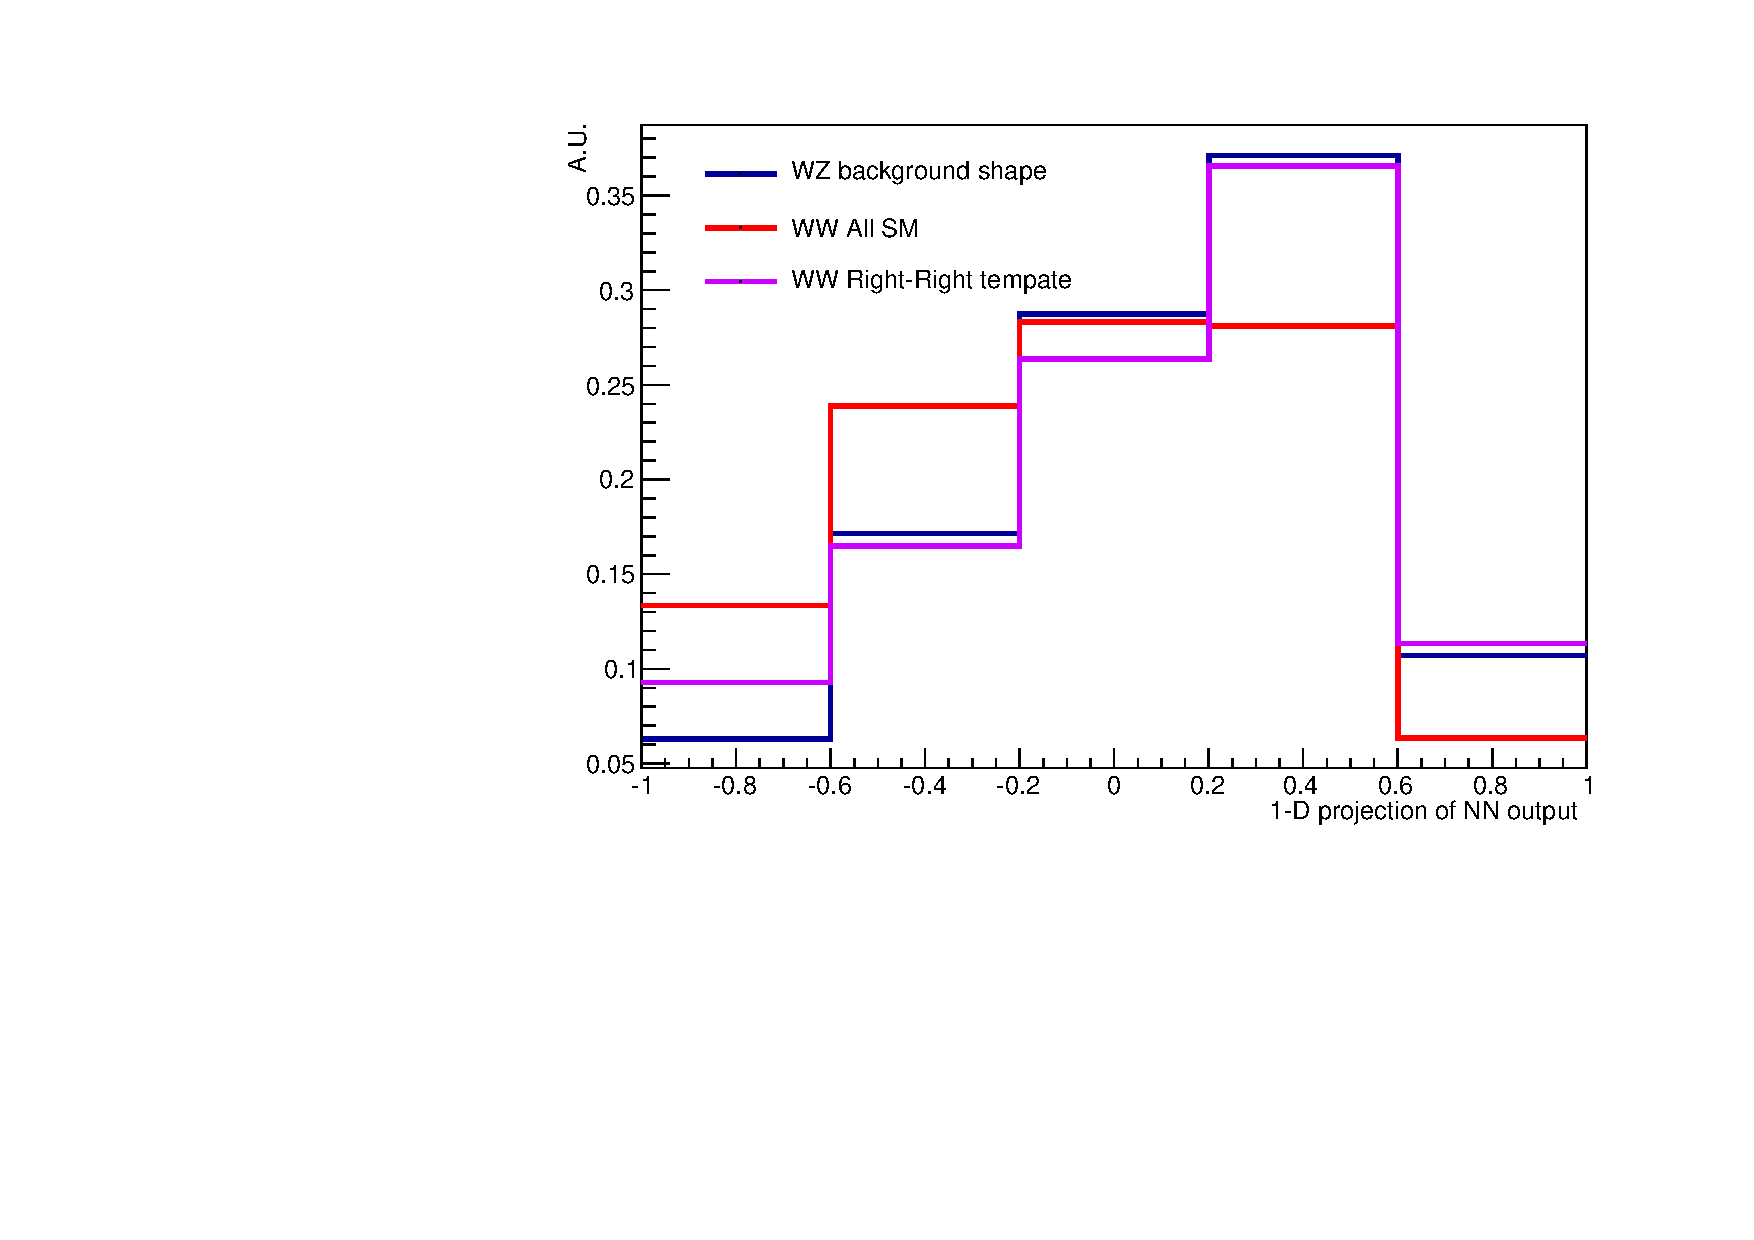
\includegraphics[width=.45\textwidth]{./fig/sig_bkg.pdf}
\caption{\label{sig_bkg} Signal and background shapes for the
  calculated $\cts$.}

\end{figure}

\section{Conclusions}
We present a method to determine the $WW$ polarization fractions in
\ssWW events by using a deep machine learning technique.  This method
allows to recover the charged lepton angular distributions in the $W$
boson rest frame from measurable event kinematics.  We compare the
results obtained from this method and from other traditional methods
to illustrate the gain in sensitivity with our method.  Cuts to reject
backgrounds as well as detector smearing reduces the sensitivity as
expected, but the method remains a useful tool for the study of
polarization fractions in VBS.

\begin{thebibliography}{99}
%\cite{Chatrchyan:2012ufa}
%\cite{Aad:2012tfa}
\bibitem{ATLAS_higgs} 
  G.~Aad {\it et al.}  [ATLAS Collaboration],
  %``Observation of a new particle in the search for the Standard Model Higgs boson with the ATLAS detector at the LHC,''
  Phys.\ Lett.\ B {\bf 716}, 1 (2012)
  [arXiv:1207.7214 [hep-ex]].
  %%CITATION = ARXIV:1207.7214;%%
  %4423 citations counted in INSPIRE as of 02 Jun 2015


\bibitem{CMS_higgs} 
  S.~Chatrchyan {\it et al.}  [CMS Collaboration],
  %``Observation of a new boson at a mass of 125 GeV with the CMS experiment at the LHC,''
  Phys.\ Lett.\ B {\bf 716}, 30 (2012)
  [arXiv:1207.7235 [hep-ex]].
  %%CITATION = ARXIV:1207.7235;%%
  %4343 citations counted in INSPIRE as of 02 juin 2015

%\cite{Aad:2014zda}
\bibitem{ATLAS_ssWW} 
  G.~Aad {\it et al.}  [ATLAS Collaboration],
  %``Evidence for Electroweak Production of $W^{\pm}W^{\pm}jj$ in $pp$ Collisions at $\sqrt{s}=8$ TeV with the ATLAS Detector,''
  Phys.\ Rev.\ Lett.\  {\bf 113}, no. 14, 141803 (2014)
  [arXiv:1405.6241 [hep-ex]].
  %%CITATION = ARXIV:1405.6241;%%
  %26 citations counted in INSPIRE as of 02 juin 2015


%\cite{Khachatryan:2014sta}
\bibitem{CMS_ssWW} 
  V.~Khachatryan {\it et al.}  [CMS Collaboration],
  %``Study of vector boson scattering and search for new physics in events with two same-sign leptons and two jets,''
  Phys.\ Rev.\ Lett.\  {\bf 114}, no. 5, 051801 (2015)
  [arXiv:1410.6315 [hep-ex]].
  %%CITATION = ARXIV:1410.6315;%%
  %6 citations counted in INSPIRE as of 02 juin 2015


%\cite{Han:2009em}
\bibitem{Han:2009em} 
  T.~Han, D.~Krohn, L.~T.~Wang and W.~Zhu,
  %``New Physics Signals in Longitudinal Gauge Boson Scattering at the LHC,''
  JHEP {\bf 1003}, 082 (2010)
  [arXiv:0911.3656 [hep-ph]].
  %%CITATION = ARXIV:0911.3656;%%
  %38 citations counted in INSPIRE as of 02 juin 2015

%\cite{Doroba:2012pd}
\bibitem{Doroba:2012pd} 
  K.~Doroba, J.~Kalinowski, J.~Kuczmarski, S.~Pokorski, J.~Rosiek, M.~Szleper and S.~Tkaczyk,
  %``The $W_L W_L$ Scattering at the LHC: Improving the Selection Criteria,''
  Phys.\ Rev.\ D {\bf 86}, 036011 (2012)
  [arXiv:1201.2768 [hep-ph]].
  %%CITATION = ARXIV:1201.2768;%%
  %11 citations counted in INSPIRE as of 02 juin 2015



%\cite{Baldi:2014kfa}
\bibitem{Baldi:2014kfa} 
  P.~Baldi, P.~Sadowski and D.~Whiteson,
  %``Searching for Exotic Particles in High-Energy Physics with Deep Learning,''
  Nature Commun.\  {\bf 5}, 4308 (2014)
  [arXiv:1402.4735 [hep-ph]].
  %%CITATION = ARXIV:1402.4735;%%
  %2 citations counted in INSPIRE as of 02 juin 2015

%\cite{Baldi:2014pta}
\bibitem{Baldi:2014pta} 
  P.~Baldi, P.~Sadowski and D.~Whiteson,
  %``Enhanced Higgs Boson to $\tau^+\tau^-$ Search with Deep Learning,''
  Phys.\ Rev.\ Lett.\  {\bf 114}, no. 11, 111801 (2015)
  [arXiv:1410.3469 [hep-ph]].
  %%CITATION = ARXIV:1410.3469;%%

\end{thebibliography}

